\documentclass[10pt,a4paper]{article}
\usepackage[utf8]{inputenc}
\usepackage[francais]{babel}
\usepackage[T1]{fontenc}
\usepackage{amsmath}
\usepackage{amsfonts}
\usepackage{amssymb}
\usepackage{graphicx}
\usepackage{enumitem}
\usepackage{lmodern}
\usepackage{listings}
\usepackage{color}
\usepackage{tikz}

\definecolor{mygreen}{rgb}{0,0.6,0}
\definecolor{mygray}{rgb}{0.5,0.5,0.5}
\definecolor{mymauve}{rgb}{0.58,0,0.82}

\lstset{ %
  backgroundcolor=\color{white},   % choose the background color; you must add \usepackage{color} or \usepackage{xcolor}
  basicstyle=\footnotesize,        % the size of the fonts that are used for the code
  breakatwhitespace=false,         % sets if automatic breaks should only happen at whitespace
  breaklines=true,                 % sets automatic line breaking
  captionpos=b,                    % sets the caption-position to bottom
  commentstyle=\color{mygreen},    % comment style
  deletekeywords={...},            % if you want to delete keywords from the given language
  escapeinside={\%*}{*)},          % if you want to add LaTeX within your code
  extendedchars=true,              % lets you use non-ASCII characters; for 8-bits encodings only, does not work with UTF-8
  frame=single,                    % adds a frame around the code
  keepspaces=true,                 % keeps spaces in text, useful for keeping indentation of code (possibly needs columns=flexible)
  keywordstyle=\color{blue},       % keyword style
  language=Java,                   % the language of the code
  morekeywords={*,...},            % if you want to add more keywords to the set
  numbers=left,                    % where to put the line-numbers; possible values are (none, left, right)
  numbersep=5pt,                   % how far the line-numbers are from the code
  numberstyle=\tiny\color{mygray}, % the style that is used for the line-numbers
  rulecolor=\color{black},         % if not set, the frame-color may be changed on line-breaks within not-black text (e.g. comments (green here))
  showspaces=false,                % show spaces everywhere adding particular underscores; it overrides 'showstringspaces'
  showstringspaces=false,          % underline spaces within strings only
  showtabs=false,                  % show tabs within strings adding particular underscores
  stepnumber=2,                    % the step between two line-numbers. If it's 1, each line will be numbered
  stringstyle=\color{mymauve},     % string literal style
  tabsize=4,                       % sets default tabsize to 2 spaces
  title=\lstname                   % show the filename of files included with \lstinputlisting; also try caption instead of title
}
\usepackage[left=2cm,right=2cm,top=2cm,bottom=2cm]{geometry}


\date{Vendredi 10 octobre 2014}
\author{Groupe 2.2}
\title{Produit Mission 2 }

\begin{document}
\maketitle

\section*{Question 1 - Henneton Romain}
\section*{Question 2 - Henneton Romain}


\section*{Question 3 - Arnaud Dethise}

	Un arbre équilibré (\textit{balanced}) est un arbre binaire dont la hauteur est minimisée. Ainsi, un arbre binaire contenant $l$ feuilles (\textit{leafs}) est équilibré s'il s'étend sur $log_{2}(l)+1$ niveaux, arrondi vers le haut.
	Un arbre binaire équilibré contenant $n$ nœuds s'étend sur $log_{2}(n+1)$ niveaux.
	
	Remarque : un arbre correspondant à cette définition est dit \textit{à critère d'équilibre partiel}. Un arbre \textit{à critère d'équilibre total} devrait aussi être complet (voir ci-après), mais est rarement utilisé car cette contrainte peut imposer une réorganisation de l'arbre entier en cas d'insertion.
	
	Un arbre propre est un arbre dans lequel tout nœud possède 0 ou 2 sous-arbres.
	Un arbre binaire équilibré n'est pas forcément propre, comme on peut le voir dans l'arbre représenté sur la figure \ref{balanced_improper_tree}.
	
	\begin{figure}[!h]
	\begin{center}
		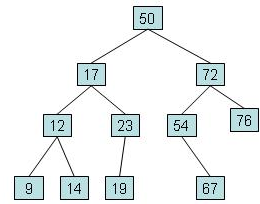
\includegraphics[scale=.7]{q3-balanced_improper_tree.png}
		\caption{Les nœuds 23 et 54 n'ont qu'un seul \textit{subtree}, l'arbre est donc impropre. Il est par contre équilibré (11 nœuds, 4 niveaux). \textit{(source csupomona.edu)}}
		\label{balanced_improper_tree}
	\end{center}
	\end{figure}
	
	Un arbre binaire essentiellement complet est un arbre pour lequel chaque niveau à l'exception du dernier est totalement rempli, et tous les nœuds du dernier niveau sont placés aussi loin que possible à gauche.
	Le fait de définir l'arbre comme \textit{essentiellement} complet signifie que le dernier niveau peut ne pas être totalement rempli.
	
	Un arbre complet est toujours équilibré car le fait de placer les nouveaux nœuds sur le niveau le plus haut possible minimise effectivement la hauteur de l'arbre.
	Un arbre équilibré n'est en revanche pas forcément complet. Un contre-exemple est donné à la figure \ref{balanced_incomplete_tree}.
	
	\begin{figure}[!h]
	\begin{center}
		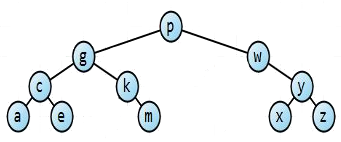
\includegraphics[scale=.7]{q3-balanced_incomplete_tree.png}
		\caption{L'arbre compte 11 nœuds et 4 niveaux, il est donc équilibré. En revanche, le niveau $n-1$ n'est pas rempli et tous les nœuds du niveau $n$ ne sont pas à gauche, l'arbre est donc incomplet. \textit{(source boyet.com, edited)}}
		\label{balanced_incomplete_tree}
	\end{center}
	\end{figure}
	
	Attention à ne pas confondre les arbres équilibrés et les arbres AVL, quasi équilibrés.


\section*{Question 4}
\section*{Question 5 - Arnaud Dethise}

	Considérons une variation de la classe LinkedBinaryTree de DSAJ ne contenant pas de méthode \textit{parent} et n'implémentant que l'interface \textit{Iterable<E>}, qui ne permet pas de parcourir l'iterator vers l'arrière.
	Cela signifie qu'il est impossible de remonter dans l'arbre, et que par conséquent chaque accès à un nœud n'appartenant pas à un sous-arbre doit se faire depuis la racine.
	Si nous voulons pouvoir nous déplacer dans l'arbre, il faut donc créer la méthode \textit{parent}, ci-après.
	
	\begin{lstlisting}
public Position<E> parent(Position<E> p) throws IllegalArgumentException
{
	Node<E> node = validate(p);
	return getParentDfs(node, root);
}

private Position<E> getParentDfs(Node<E> node, Node<E> hook)
{
	if (hook == null) return null;
	else
	{
		if (node == hook.getLeft() || node == hook.getRight()) return hook;
		else
		{
			Node<E> tmp;
			tmp = getParentDfs(node, hook.getLeft());
			return (tmp != null ? tmp : getParentDfs(node,hook.getRight()));
		}
	}
}
	\end{lstlisting}
	
	Cet algorithme parcourt dans le pire cas une fois chaque nœud de l'arbre, et a donc une complexité temporelle O(n), n étant le nombre de nœuds dans l'arbre.

\section*{Question 6 - Gil De Grove}
\lstinputlisting{LinkedRBinaryTree.java}
\section*{Question 7}
\section*{Question 8}
\clearpage
\section*{Question 9 - Zacharie Kerger}

Chaque arbre représente la dérivée formelle de l'expression présente à sa gauche.\\

\textbf{(f + g)' =} 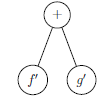
\includegraphics[scale=1]{q9-f+g.png}
\textbf{(f - g)' =} 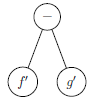
\includegraphics[scale=1]{q9-f-g.png}
\textbf{(f * g)' =} 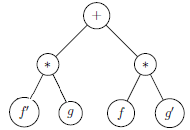
\includegraphics[scale=1]{q9-fg.png} \\
\textbf{($\frac{f}{g}$)' =} 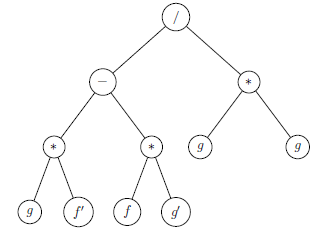
\includegraphics[scale=1]{q9-fdivg.png}
\textbf{sin(f)' =} 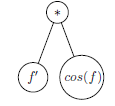
\includegraphics[scale=1]{q9-sinf.png} \\
\textbf{cos(f)' =} 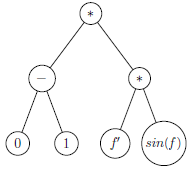
\includegraphics[scale=1]{q9-cosf.png}
\textbf{($f^{a}$)' =} 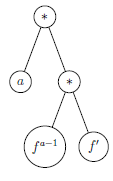
\includegraphics[scale=1]{q9-fa.png}\\
\textbf{($\frac{1}{g}$)' =} 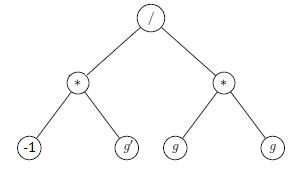
\includegraphics[scale=1]{q9-1divg.png}

\end{document}
